\documentclass{article}%
\usepackage[T1]{fontenc}%
\usepackage[utf8]{inputenc}%
\usepackage{lmodern}%
\usepackage{textcomp}%
\usepackage{lastpage}%
\usepackage[head=40pt,margin=0.5in,bottom=0.6in]{geometry}%
\usepackage{graphicx}%
%
\title{\textbf{Habitantes de Maracaibo protestan por tener 10 días sin luz}}%
\author{EL NACIONAL WEB}%
\date{10/10/2018}%
%
\begin{document}%
\normalsize%
\maketitle%
\textbf{URL: }%
http://www.el{-}nacional.com/noticias/protestas/habitantes{-}maracaibo{-}protestan{-}por{-}tener{-}dias{-}sin{-}luz\_255200\newline%
%
\textbf{Periodico: }%
EN, %
ID: %
255200, %
Seccion: %
Protestas\newline%
%
\textbf{Palabras Claves: }%
Protestas, Sociedad\newline%
%
\textbf{Derecho: }%
2.8, %
Otros Derechos: %
, %
Sub Derechos: %
2.8.1\newline%
%
\textbf{EP: }%
SI\newline%
\newline%
%
\textbf{\textit{Las personas piden a las autoridades de Corpoelec que restablezcan el servicio eléctrico~}}%
\newline%
\newline%
%
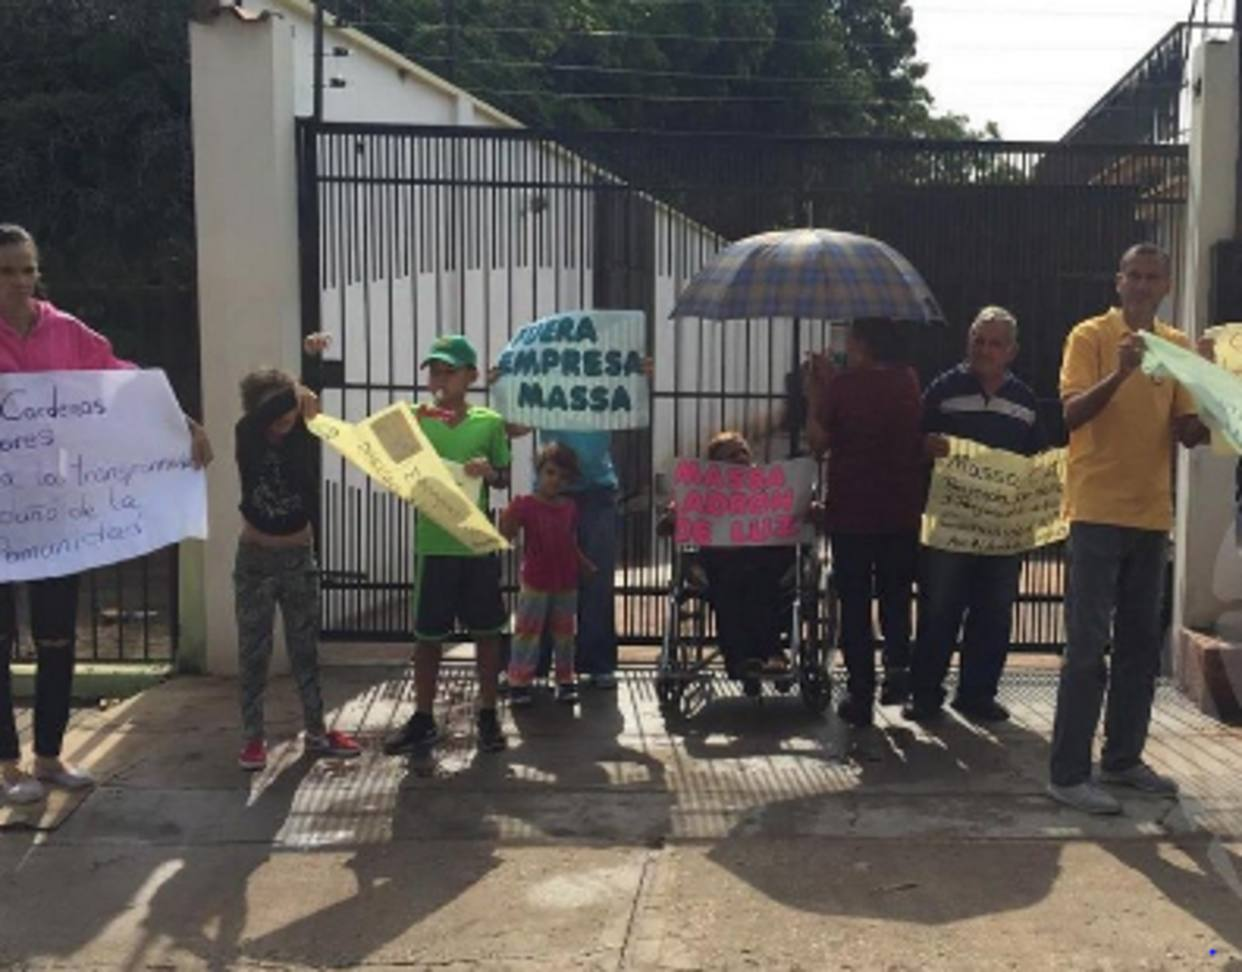
\includegraphics[width=300px]{18.jpg}%
\newline%
%
Habitantes del estado Zulia protestan este miércoles porque aseguran que tienen 10 días sin luz.%
\newline%
%
Las personas pertenecen a la parroquia Raúl Leoni, de la ciudad de Maracaibo y~piden a las autoridades de Corpoelec solucionar el problema eléctrico a la brevedad posible.%
\newline%
%
\end{document}